%% ----------------------------------------------------------------
%% Thesis.tex -- MAIN FILE (the one that you compile with LaTeX)
%% ---------------------------------------------------------------- 

% Set up the document
\documentclass[a4paper, 11pt, oneside]{Thesis}  % Use the "Thesis" style, based on the ECS Thesis style by Steve Gunn
\graphicspath{{Figures/}}  % Location of the graphics files (set up for graphics to be in PDF format)

% Include any extra LaTeX packages required
\usepackage[square, numbers, comma, sort&compress]{natbib}  % Use the "Natbib" style for the references in the Bibliography
\usepackage{verbatim}  % Needed for the "comment" environment to make LaTeX comments
\usepackage{vector}  % Allows "\bvec{}" and "\buvec{}" for "blackboard" style bold vectors in maths
\usepackage{xcolor}
\usepackage{slashbox}
\usepackage{enumitem} %Continue enumerations
\usepackage{listings} %For source code framse
\usepackage{float}
\usepackage[toc,page]{appendix}
\hypersetup{urlcolor=black, colorlinks=false}  % Colours hyperlinks in blue, but this can be distracting if there are many links.
%Listings
\colorlet{light-gray}{gray!20}
\lstset{ breaklines=true,
		backgroundcolor=\color{light-gray},
		breakatwhitespace=false,
		frame=single,
		language=Octave} 

%% ----------------------------------------------------------------
\begin{document}
\frontmatter      % Begin Roman style (i, ii, iii, iv...) page numbering

% Set up the Title Page
\title  {Depth perception: Effects of Head Tracking in Analysing
Graphs in
3D}
\authors  {          
			Allegretta, Mauro \\
			Ambite, Diego \\
			Lozano, Francisco J. \\
			Rinsma, Thomas 
            }
\addresses  {\groupname\\\deptname\\\univname}  % Do not change this here, instead these must be set in the "Thesis.cls" file, please look through it instead
\date       {\today}
\subject    {}
\keywords   {}

\maketitle

%% ----------------------------------------------------------------

\setstretch{1.3}  % It is better to have smaller font and larger line spacing than the other way round

% Define the page headers using the FancyHdr package and set up for one-sided printing
\fancyhead{}  % Clears all page headers and footers
\rhead{\thepage}  % Sets the right side header to show the page number
\lhead{}  % Clears the left side page header

\pagestyle{fancy}  % Finally, use the "fancy" page style to implement the FancyHdr headers


%% ----------------------------------------------------------------
\lhead{\emph{Contents}}  % Set the left side page header to "Contents"
\tableofcontents  % Write out the Table of Contents

%% ----------------------------------------------------------------
% End of the pre-able, contents and lists of things
% Begin the Dedication page

\setstretch{1.3}  % Return the line spacing back to 1.3

\addtocontents{toc}{\vspace{2em}}  % Add a gap in the Contents, for aesthetics


%% ----------------------------------------------------------------
\mainmatter	  % Begin normal, numeric (1,2,3...) page numbering
\pagestyle{fancy}  % Return the page headers back to the "fancy" style

% Include the chapters of the thesis, as separate files
% Just uncomment the lines as you write the chapters

\lhead{\emph{Introduction}} 
\chapter{Introduction}

Many research about Virtual Reality has proved that the combination of
perspective stereoscopic view and tracking the position in real time of
the user as he moves is a good idea to visualizing 3D scenes. One of the
papers that has gone deeper in the topic of visualizing 3D objects using
VR is \emph{Evaluating Stereo and Motion Cues for Visualizing
Information Nets in Three Dimensions \cite{ware1996evaluating}}.

The main goal for this project is to replicate one of the experiments
carried out in the mentioned paper. This experiment consists of
analyzing the difference between user comprehension of network graphs
(1) in 2D versus 3D and (2) with and without head-tracking. This
difference will be measured by having the user perform a simple task and
recording several metrics such as timing and error rate. As a result of
the experiment, we hope to be able to make conclusions about whether 3D
vision and/or (lack of) head-tracking is better for the comprehension of
visualized graphs.

In addition to the metrics proposed in the experiment, we will try to
gain more insight of the effects of 3D vision and head-tracking by
measuring additional metrics such us the distance traversed or the
amount rotated by the head or the distance that the subject traverses
inside the virtual environment. The purpose of these additional metrics
is to test whether or not there exists a correlation between the
complexity of the graph and the amount of movement that is required for
the subject to comprehend it. Of course, our purpose is not to provide a
completely general answer about how much is gained by using
head-tracking because its use is task specific. The conclusions will
only try to generalize a hypothetic application in real life for
visualizing graphs and they should not be considered as applicable in
all the scenarios where head-tracking is used.

As students, we are conscious that many problems may appear during the
development of the project and we will have to overcome some
difficulties that could lead to the failure of the experiment. Some of
these difficulties are:

\begin{itemize}
\item
  Retrieve some metrics from Oculus Rift and get used to the Unity
  framework.
\item
  Design appropriate levels (of difficulty) for our analysis purpose in
  order to get useful data.
\item
  Interpret the data correctly to extract truthful and correct
  conclusions.
\item
  Technical difficulties/limitations regarding frame rate, graphics
  rendering, etc.
\end{itemize}

All these risks are taken into account and the priority of this study is
not only to understand some of the topics we have seen in class but also
see the difficulties that imply to deal with a Virtual Reality
experiment.

To define a guideline for our experiment, we have defined a series of
questions that we will try to give answer:

\begin{itemize}
\item
  Is it better in terms of comprehension to visualize network graphs in
  2D or 3D?
\item
  Does head-tracking help increase this comprehension in addition to 3D
  vision?
\item
  Do these differences become bigger as we increase the complexity of
  the graph?
\item
  How similar are the obtained results to those in the original paper?
\end{itemize}

Therefore, we will try to provide quantitative measures that could prove
how much more a graph can be understood in 3D with respect to 2D. At the
end of the report, we should give strong reasons about if using 3D
graphics and virtual reality is a good combination to interact with
information structures.
 % Introduction

\lhead{\emph{Related Work}} 
\chapter{Related Work}

As mentioned in the previous section, this experiment is an
extension of the one proposed in the study \emph{Evaluating Stereo and
Motion Cues for Visualizing Information Nets in Three Dimensions.}
Despite the fact that the paper of Ware and Franck is a good reference for comparing
our conclusions to, we must consider the context and the
technology used for their experiment. Their paper was published in
1996, when virtual reality started to be used in some applications but
the technology was not very advanced in this area and a lot of research
tried to show the possible future applications it may have in the next
decade. The hardware used in the paper consisted of 3D LCD shutter
glasses that provided the stereo vision and an ultrasonic head-tracking
device embedded inside the frame of the glasses. The monitors used for
the experiment ran at 120Hz and each eye received a 60Hz update rate
using the shutter glasses.

Of course, a great advanced in technology has happened since 1996, and
twenty years later, more sophisticated technology is available and this is
an important factor that we cannot overlook. For our experiment, we use the 
Oculus Rift Development Kit 2. This device has a resolution of 960x1080 pixels
per eye, a low-persistence OLED display, positional tracking, a higher
refresh rate than previous versions of Oculus Rift (Up to 75 Hz) and an
external HDMI port.

The difference in technology is one of the main differences between our
experiment and Ware and Franck's experiment. Additionally we introduced some
differences in the conditions and the variables of the experiment. In
the original paper, four different combinations in the type of
visualization are carried out: 2D, 2D and head tracking, 3D and 3D and
head tracking. However, in our experiment, only three conditions are
tried: 2D, 3D and head tracking, and a combination of 3D, head tracking
and partial visual reduction. This last condition could not be performed
due to technical issues with the development framework and the time
constraints of the experiment.

Moreover, the variables taken into account for performing the experiment
also changed. In the original paper, the number of nodes are varied to
measure the error rate and the time taken by the subjects. They
extract conclusions about performance using these metrics. On the other
hand, we used a different approach for obtaining different results.
Instead of the raw number of nodes an abstraction called
\textbf{complexity level} is used instead. This abstraction takes into account
the number of nodes and the minimum and maximum
degree that each node can have. This degree for each node varies randomly between these values
but the number of nodes is fixed for each complexity level. Using
different types of complexity levels, we tried to simulate different
scenarios of complexity and to meassure how much does it affects the error rate
and employed time until the user gives an answer.

Finally, the head movement is also taken into account. We use a distance
metric provided by the Unity framework in the virtual space that allows us
to compare relatively between different amounts of movement. This variable is new
in respect to the original paper and it's interesting to analyze because in
may provide information about how head-tracking affects the behavior of
the subjects.

 % Related Work

\lhead{\emph{Experiment}} 
\chapter{Experiment}

\section{General description}\label{general-description}

The experiment has been design with the main purpose of collecting relevant
and consistent data from the Oculus Rift device and the subjects
regarding the effects of stereoscopic vision and head tracking in the
task of 3D graph comprehension. In addition, we will create a series of
scenarios to retrieve data regarding the effects of visual memory in
3D graph comprehension when the range of vision is reduced.

The experiment will be composed of \textbf{three stages}. Each one will
be composed of \textbf{three scenarios} according to the graph
complexity\textbf{.} The stages are defined as follows:

\begin{enumerate}
\def\labelenumi{\arabic{enumi}.}
\item
  \textbf{Stage 1}: The subject performs the experiment in each scenario
  directly on the screen of a laptop. For this stage, no Oculus Rift
  device will be used and the subject will be able to visualize the
  graph looking at the screen, with no head tracking enabled.
\item
  \textbf{Stage 2}: The subject performs the experiment in each scenario
  using the Oculus Rift device. Head tracking will be active and there
  will not be any kind of reduction of the angle of vision.
\item
  \textbf{Stage 3}: The subject performs the experiment in each scenario
  using the Oculus Rift device, Head tracking will be active and there
  will be a reduction of \textasciitilde{}50\% of the range of vision
  both in the horizontal and in the vertical axis.
\end{enumerate}

Each stage will be composed of three scenarios with \textbf{challenges}
whose level of difficulty goes from 1 to 3. A challenge will consist of
answering whether or not there exists a 2-length path connecting two highlighted
nodes. Each challenge will have a 50\% of probability of containing such
a path. The subject will have to answer (yes or no) whether or not this
path exists before the maximum time for the challenge is over. If the
user has not made a decision before the time is over, it will count as a
fail.

Each scenario will contain a graph with
different complexity in increasing order. Due to the difficulty to
determine the number of nodes and edges that fit best with each level of
complexity, some testing will still be performed using different number
of nodes and edges, and differing numbers of minimum an maximum degree per node,
to design three complexity levels that have distinct
average times needed to solve the problem in the experiment.

The estimated mean time to complete the three stages will depend on the
maximum time we define for each level of complexity but it will not be
more than 10 minutes. The estimated time for each stage will be in a
range between 1 and 3 minutes with a mean time of 1 minute for each
stage.

Finally, the experiment will be allowed to be repeated several times by
a subject. The first attempt will be considered for the main study and
the consecutive attempts will be taken into account for a possible
secondary study about the adaptive process in each stage.

\section{Constraints}\label{constraints}

For this experiment, we have defined some rules and constraints that
will delimit the experiment's boundary and specify clearly what the
subject can or can't do. The constraints are the following:

\begin{itemize}
\item
  A maximum amount of time will be defined for each level of complexity.
  The range of maximum time will be somewhere between 10 seconds and 1
  minute. This is an approximation and could be modified after the
  implementation of the experiment.
\item
  If the subject runs out of time for one level, the next level or stage
  will start and the challenge will be treated as failed.
\item
  The subject won't be allowed to stand up from the chair. He will be
  able to rotate his head and move it in any direction though.
\item
  A subject will be allowed to repeat the experiment a maximum of 3
  times to avoid virtual reality sickness.
\item
  The subject will sit in a range between 60 centimeters and 1 meter in
  front of the laptop screen for Stage 1.
\item
  If the subject interrupts the experiment without completing all the
  stages and levels, the results will be discarded.
\item
  The subject won't be allowed to take off the Oculus Rift in Stages 2
  and 3. If the subject takes off the OR during these stages, the
  experiment will be interrupted and the data collected will be
  discarded.
\item
  The subject won't be provided with any joystick to move inside the
  scenarios. He will have access to the mouse and/or keyboard to provide
  a yes or no answer to each experiment.
\end{itemize}

\section{Research questions}\label{research-questions}

In this section we are defining the different approaches that we will
use to answer the research questions with the data collected in the
experiment. The proposed research questions are the following ones:

\begin{itemize}
\item
  \emph{Does stereoscopy and head tracking add to a person's
  comprehension of 3D graphs?}
\end{itemize}

This question will be answered using the data collected from Stages 1
and 2. We will compare the difference of performance in terms of time
and error rate. In addition, the subject will be asked at the end of the
experiment to rate the experience in each stage. Data collected in these
two stages will be compared among them to see if these techniques are
really helpful and how much are they in terms of performance.

\begin{itemize}
\item
  \emph{Does there exist any correlation between the amount of head
  movement and the graph complexity when 3D graphs are visualized with a
  virtual reality device?}
\end{itemize}

This question will be answered using the data collected from Stages 2
and 3. We will measure the distance traversed by the head for each
scenario and use this metric to see if the distance increases
proportionally to the complexity of the graph.

\begin{itemize}
\item
  \emph{How important is the range of vision in comprehension of 3D
  graphs with stereoscopic vision? Does visual memory have any influence
  in the comprehension of 3D graphs?}
\end{itemize}

The second question is the hardest one because it depends on many
factors that are hard to measure without special equipment. However, our
approach of reducing the range of vision of the graph could give us some
idea of how large the difference in the performance is in this scenario.
We hypothesize that the reduction of the range of vision in Stage 3 will
make the subject look several times in different directions to construct
a memory image of the graph. This probably takes a certain amount of
time that we will compare with the results obtained in Stage 2.
Analysing the results, we will try to form a conclusion on how
significant the use of visual memory is in the comprehension of 3D
graphs.

\begin{itemize}
\item
  \emph{How similar are the obtained results with the findings in the
  original paper?}
\end{itemize}

This question will be answered using the data collected from Stages 1
and 2 and once the first question has been answered. We will make a
comparison between the conclusions of our experiment and the  original paper and we will try to
explain any differences if they are significant enough.


 % Experiment

\lhead{\emph{Results}} 
\chapter{Results}

The experiment was performed 16 times with 6 different people. The
results were analyzed, taking into account the previous descripted metrics
and different perspectives that are reflected in the following 5
plots that are commented on individually.

\begin{figure}[!ht]
\centering
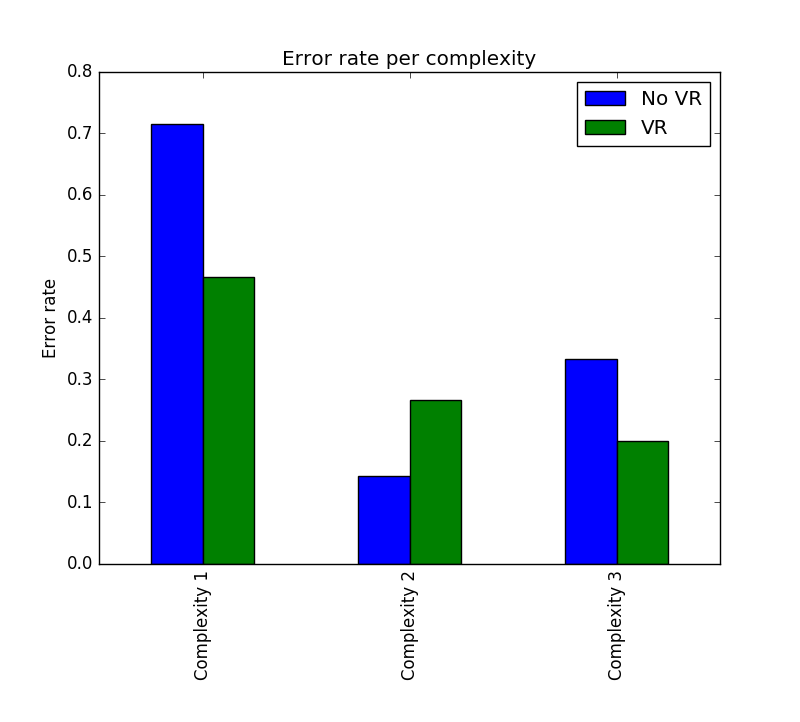
\includegraphics[scale=0.33]{image1.png}
\caption{Error rate per complexity level and condition} \label{fig:plot1}
\end{figure}

Figure \ref{fig:plot1} shows how the X axis is split up in three complexity
levels and the Y axis measures the average error rate in each complexity
level. The first interesting thing that can be observed in this plot is
that in the first and third complexity levels, the error rate produced
with no use of VR is higher than the error rate when the subjects used
VR to visualize the graph. This was expected because the use of VR
should make the task of visualizing graphs easier. However, in the
second complexity level the exact opposite happens. This result was
completely unexpected and it's difficult to make a conclusion about this
distortion.

If we take the mean percentage of correct answers, that is the
inverse of the error rate, the percentage that corresponds to the use of
VR is 68.89\%. This is slightly higher than the percentage of correct
answers without the use of VR, which is 60.47\%. This is not a big
difference in performance, but follows the tendency meassured in the
original paper.

On the other hand, independently of whether VR is used or not, the error rate in the
first complexity level is quite a lot higher than in the other two complexity
levels. This is the opposite of what we expected and what was found in
the original paper. That is, the error rate should increase
proportionally to the level of complexity. The explanation we can give for
this is that the subjects that perform the experiment for the first time
must get used to the device and the experiment, thereby taking longer in the first few attempts. This learning process takes some time that we didn't provide. Therefore, we could say
that this was an issue caused by the lack of familiarity with the device
and an issue in the design and execution of the experiment.

\begin{figure}[!ht]
\centering
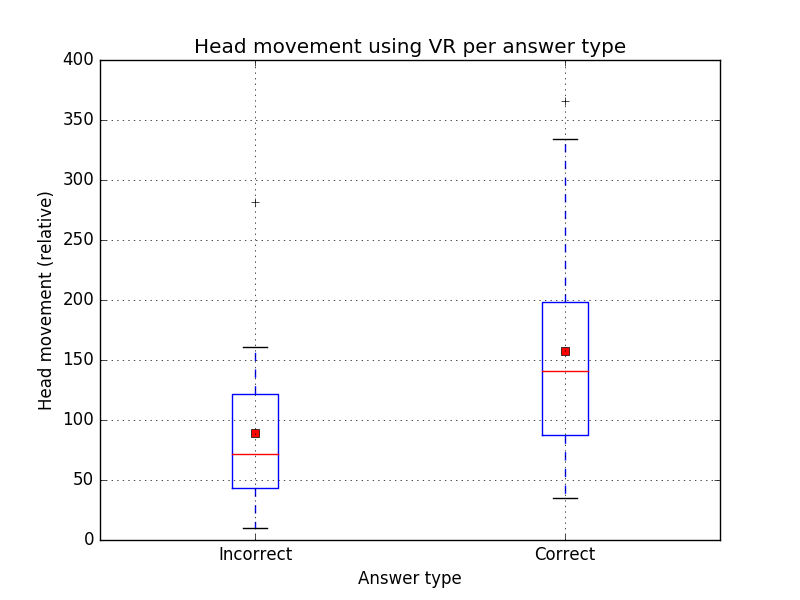
\includegraphics[scale=0.33]{image2.png}
\caption{Head movement using VR per answer type} \label{fig:plot2}
\end{figure}

In figure \ref{fig:plot2}, we can see the amount of head movement produced every time
a subject provided either an incorrect or a correct answer. This
relation wasn't discussed in the original paper and it provided some
interesting results. The main result was that the amount of head
movement increased by 30.19\% for correct answers with respect to
incorrect answers. That is, people that move their head more to
visualize the graph are more likely to give the correct answer. The head
movement was measured using the movement of the camera in the virtual
space in Unity units. It doesn't provide a reference to see the
real distance traversed by the head in meters, but it allows us to
compare among different scenarios and subjects.

\begin{figure}[!ht]
\centering
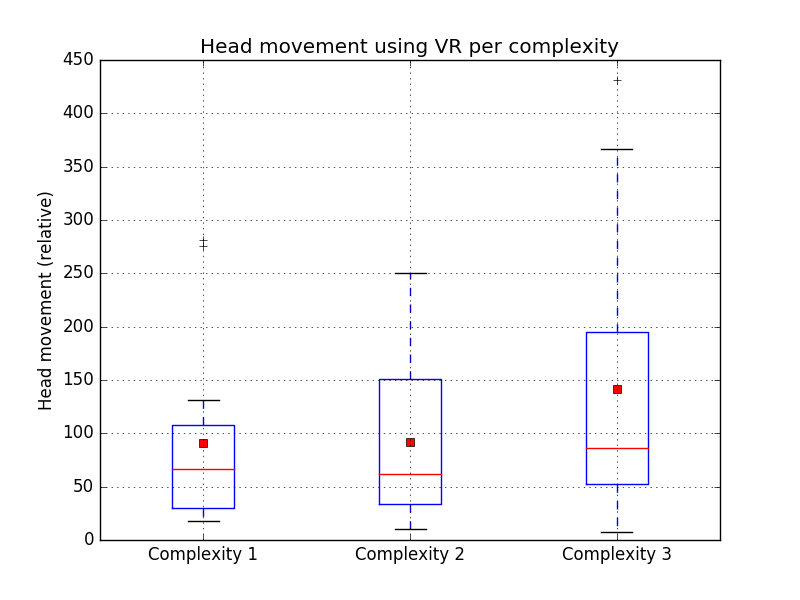
\includegraphics[scale=0.33]{image3.png}
\caption{Head movement using VR per complexity level} \label{fig:plot3}
\end{figure}

Similarly to the previous plot, in figure \ref{fig:plot3}  we can observe again the head movement in the
Y axis and the X axis is split up in three complexity levels. Specifically
for the third complexity level, the mean amount of head movement is
slightly higher than in the others. This was expected because the
experiment was set up such that subjects in higher complexity levels have
a higher maximum amount of time and thus, they tend to spend more time
and it results in a higher amount of head movement in total, on average (which follows from time, assuming a constant amount of movement per unit of time). It can be
seen as well that the variance is very high in the third complexity level
due presumably to the fact that people really liked the sensation of VR at
this point of the experiment and they moved their heads to take
advantage of the experience.

\begin{figure}[!ht]
\centering
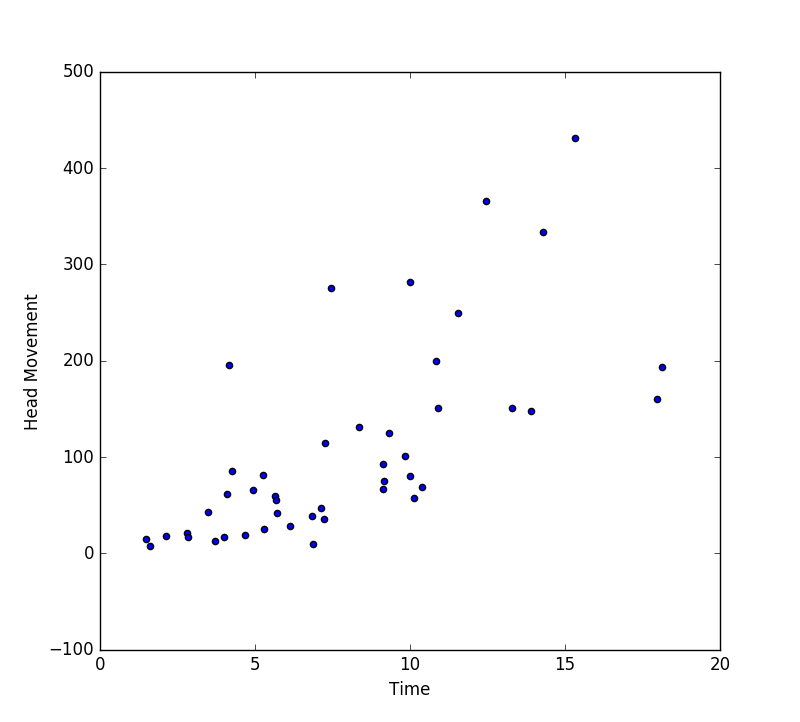
\includegraphics[scale=0.33]{image5.png}
\caption{Head movement and response time (in seconds)} \label{fig:plot5}
\end{figure}

In the scatter plot of figure \ref{fig:plot5} we can observe the same pattern of the previous
plot. Almost all the points are clustered in a range between 0 and 10
seconds and almost all of them have an upper bound of 100 units of head
movements. From this point, the variance starts to grow exponentially as
the time increases. This reaffirms the conclusion that when
people have more time to give an answer, they try to see the graph from
a different perspective to be sure that they are providing a correct
answer. Therefore. in scenarios where time is less of a constraint to
visualize the graph, people uses head tracking more to better comprehend
the graph.

\begin{figure}[!ht]
\centering
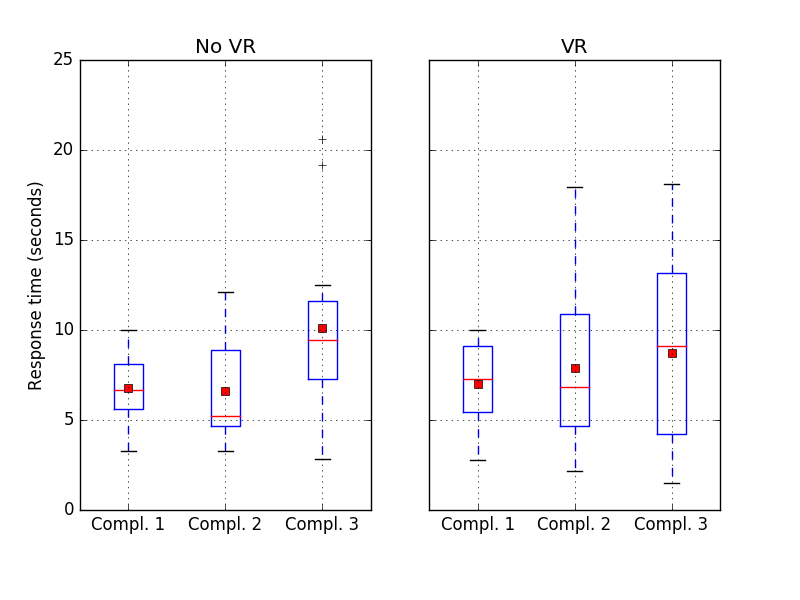
\includegraphics[scale=0.33]{image4.png}
\caption{Response time per complexity level} \label{fig:plot4}
\end{figure}

In the two box plots that are drawn in figure \ref{fig:plot4}, we can see the response time in seconds in the Y
axis, separated firstly in VR and no VR and secondly in the three
complexity levels. We can see for both plots that the higher the graph
complexity is, the higher the time a subject takes to answer. This
was of course expected because as the maximum time to answer increases,
people feel less pressure to make a decision. Therefore, we can't be
sure if the graph is really comprehended better or if it just
depends on the maximum amount of time provided to answer. This should
be compared with another version of the experiment in which the
information about the maximum amount of time is not provided and see the
real evolution.

We can also see that the variance in the response time is very high
again when VR is used. Again, we think that this is caused because
people really liked the VR experience and some of them spent longer on the experiment.
However if we observe the means and we compare them,
we can observe they are both practically the same in VR (7.81 seconds)
and No VR (7.88 seconds). Comparing to the paper, this is not what we
expected, which is that the response time should be lower when VR is used.

In all the plots we have analyzed, we can observer a common problem: The
sample size is too low to make significant conclusions. Several
technical problems and constraints in the availability of the device led
us to a partial failure in the data collecting. Some of the conclusions
we have made follow the tendency of the ones made in the provided
paper, but our results don't anywhere near the same level of significance as
those in the original paper.

For future work, if this experiment would be repeated, we would tweak
some of the parameters like the maximum amount of time to answer and the graph complexity increments, in addition to clearly informing the user about these values. Secondly, we would try to collect a much larger amount of data to get significant and reliable results that can really be compared to those in the original paper. Lastly, we would give our subjects some dry runs of the experiment, and time to get used to it. We would let them do more challenges per stage, and we would interview them about their experience afterwards.



 % Results

\lhead{\emph{Conclusions}} 
\chapter{Conclusions}

This experiment led us to face several problems and to learn the right
approach to analyze a research purpose. The first conclusion that we
draw is that the actual results are rather more different from the ones
we expected. We can explain this due to several factors that depends
both on the experiment constraints and the behavior of the subjects.
Analyzing the results statistically, we assert that the distortion from
our expections could be due to the small size of our dataset. This issue
could not be foreseen at the beginning of the experiment because of the
uncertainties on the ideal set of subjects, but it turned to be a
problem at the end.

The second conclusion is that Virtual Reality offers as many solutions
as challenges to face. Dealing with the deadline for this experiment was
very challenging because of the technical issues related to the
compatibility of the Oculus SDK and the Unity framework. This compelled
us to submit the test to a little number of people and limited our
capacity to extract significant conclusions from the dataset.

Moreover, the limited time affected the behaviors of the subjects. Some
of them misenderstood the task to accomplish, influencing negatively the
results or forcing us to discard the tests. On the other hand the
subject that was able to accoplish the tasks increased his performances
with the growth of the difficulty. This was an unpredictable training
process that we didn't take into account. The second unexpected process
was the tendency of the subjects to expend more time to enjoy the VR
experience, and not because of it helped in the comprehension of the
graph, producing some distortions on the data

Despite the difficulties, we have derived two conclusions from the data:
VR and 3D vision with headtracking affects positively the visualizations
of 3D graphs and subjects prefer immersive environment and within it
they obtain better performances. Thanks to the problems we faced, we
spreaded our knowledge not only about software development (Unity
developing, Oculus Rift Hardware, Computer Graphics basics etc.) but
especially about science (scientifically approach, experimental issues,
recuiting subject, evaluating other experiments, being subjects of other
groups etc.).

Finally we thought about some possible applications of this results in
case they are supported by a bigger number of data and a more solid
scientific approach. This kind of experiment could be implemented in the
diagnosis and the treatment of neurogical deseases and in the rehab
processes measuring the level of the interactions of the patients and
their improvements during the period. In this scenario would be also
useful the third stage of our experiments that would try to analyze the
effect on the visual memory of a restricted field of view.





 % Conclusions

\begin{appendices}

\chapter{Implementation}

For the implementation of this experiment, we have used Unity framework
and Oculus Rift SDK. A controller class was in charge of controlling the
experiment flow across the different stages and scenarios. The
controller contained an internal timer that controlled the remaining
time for each scenario. The set of rules, such as maximum time and
reduction of range of vision, used for each stage are stored in a data
structure.

The only interaction allowed with each scenario was provided through the
mouse. The subject will use the left mouse button to answer that the
there exists a 2-length path between the highlighted nodes and the right
mouse to give a negative answer. The rest of the interactions such as
initiating the timer, change the scenarios or reduce the angle of vision
is done through the controller and no movement is implemented inside the
scenario.

The graphs were randomly generated for each scenario using some defined
constants according to the level of complexity of the graph. Some of
this constants were the number of edges and nodes and the probability of
generating a 2-length path between two points. The graph was undirected,
with white edges connecting blue nodes. The highlighted points were
drawn in red and the background of the scenario will be black to improve
the visibility of the graph. Finally, all the results collected were
exported to a CSV file and analyzed using Python and matplotlib library. % Appendix

\end{appendices}


\addtocontents{toc}{\vspace{2em}}  % Add a gap in the Contents, for aesthetics
\backmatter

%% ----------------------------------------------------------------
\label{Bibliography}
\lhead{\emph{Bibliography}}  % Change the left side page header to "Bibliography"
\bibliographystyle{unsrtnat}  % Use the "unsrtnat" BibTeX style for formatting the Bibliography
\bibliography{Bibliography}  % The references (bibliography) information are stored in the file named "Bibliography.bib"


\end{document}  % The End
%% ----------------------------------------------------------------